% Use regular document class for writing it, then IEEEtran
%\documentclass[10pt,journal]{IEEEtran}\def\TBLWIDA{15mm}\def\TBLWIDB{60mm}
 \documentclass[12pt]{article} \usepackage[margin=3cm]{geometry} \usepackage[margin=20pt,font=small,labelfont=bf]{caption}\def\TBLWIDA{35mm}\def\TBLWIDB{95mm}
\usepackage[T1]{fontenc}
\usepackage[utf8]{inputenc}
\usepackage{tikz}
\usepackage{tabularx}
\usepackage{bm}
\usepackage[section]{placeins} % don't let figures cross section barrier
\usepackage{comment}
\usepackage{amsfonts}
\usetikzlibrary{calc,arrows,shapes,positioning,patterns,decorations.pathmorphing,decorations.text,intersections}
\usepackage[american,siunitx]{circuitikz}
\usepackage{subcaption}
\usepackage{siunitx}
% Shouldn't be required, but subcaption seems to override IEEEtran captions
\captionsetup{font=small,labelfont={bf}}

\newcommand{\TODO}[1]{{\bf TODO: #1}}
% Maximum three authors for IEEE
%\newcommand{\ifmaxthree}[2]{#1}
\newcommand{\ifmaxthree}[2]{#2 {\em et al}; }

%%% Macros
\newcommand\Fref[1]{Fig.\ \ref{#1}}
\newcommand\fref[1]{fig.\ \ref{#1}}
\newcommand\boxtext[2]{%
    \raisebox{#1}{\fbox{\parbox[t]{16mm}{\centering %
\textsf{\small #2}%
    }}}%
}
\newcommand\boxarrow{%
    \raisebox{-3mm}{\large $\Rightarrow$}
}
\newcommand{\JV}{\vec{J}}
\newcommand{\EV}{\vec{E}}
\newcommand{\BV}{\vec{B}}
\newcommand{\xV}{\vec{x}}
\newcommand{\xB}{\mathbf{x}}
\newcommand{\xH}{\hat{\mathbf{x}}}
\newcommand{\xT}{\tilde{\mathbf{x}}}
\newcommand{\yB}{\mathbf{y}}
\newcommand{\yT}{\tilde{\mathbf{y}}}
\newcommand{\vB}{\mathbf{v}}
\newcommand{\DB}{\mathbf{D}}
\newcommand{\IB}{\mathbf{I}}
\newcommand{\MB}{\mathbf{M}}
\newcommand{\RB}{\mathbf{R}}
\newcommand{\PB}{\mathbf{P}}
\newcommand{\QB}{\mathbf{Q}}
\newcommand{\WB}{\mathbf{W}}
\newcommand{\VB}{\mathbf{V}}
\newcommand{\JB}{\mathbf{J}}
\newcommand{\sG}{\bm{\sigma}}
\newcommand{\SG}{\bm{\Sigma}}
\newcommand{\Ew}{\mathop{\rm E}_w}


\begin{document}
\title{Electrical Impedance Tomography:\\ Tissue Properties to Image Measures}
\author{Andy Adler, Alistair Boyle
\thanks{AA is with Systems and Computer Engineering, Carleton University, Ottawa, AB is with Electrical Engineering and Computer Science, University of Ottawa}
}
\date{}
\maketitle

\begin{abstract}
Electrical Impedance Tomography (EIT) uses electrical
stimulation and measurement at the body surface to
image the electrical properties of internal tissues.
It has the advantage of a non-invasiveness and
high temporal resolution but suffers from poor spatial
resolution and sensitivity to electrode movement and
contact quality.
EIT can be useful to applications where there are conductive contrasts between
tissues, fluids or gasses, such as imaging of cancerous
or ischemic tissue or the functional monitoring
of breathing, blood flow, gastric motility
and neural activity.
The past decade has seen clinical application and commercial
activity using EIT for ventilation monitoring.
Clinical interpretation of EIT-based measures is complex, and
this review paper focuses on 
describing the image interpretation ``pathway'', from:
{\em Tissue Electrical Properties},
{\em EIT Electrodes \& Hardware},
{\em Sensitivity},
{\em Image Reconstruction},
{\em Image Processing}
to 
{\em EIT Measures}.
The relationship is discussed between the 
clinically-relevant parameters and measured or
reconstructed properties, and 
an overview given of areas of EIT application,
and our perspectives for
research and development.
\end{abstract}

%\begin{keywords}
%Electrical Impedance Tomography,
%\end{keywords}

\section{Introduction}
\TODO{
  - cite Wolf
  - cite Brazil system
  - fix openoffice
  - upload code to eidors - do we want it there?
}

Electrical Impedance Tomography (EIT) is a technique to 
image the electrical properties within a body using
electrical stimulations and measurements applied at electrodes
on the body surface.
EIT is useful when the
anatomical or physiological phenomena of interest
create contrasts in the tissue electrical properties.
Examples of anatomical contrasts are 
the differing electrical impedance spectrum of
cancerous \cite{Jossinet1998Breast} and
ischemic \cite{Packham2012Frequency} tissues.
Functional contrasts are created by changes
in the conductivity of tissue or movement of
conductively contrasting fluids or gasses, such as during
breathing, blood flow, digestive or nervous activity.

As a medical imaging modality, EIT offers several advantages:
the non-invasive attachment to a patient with electrodes and wires
is convenient for continuous monitoring applications;
it does not use ionizing radiation;
it is capable of functioning at high frame rates giving
good temporal resolution; and
it is potentially inexpensive, using off-the-shelf low frequency electronics components. 
On the other hand, EIT has poor spatial resolution, and 
is prone to artefacts from electrode
movement and poor contact quality.


%\subsection{Brief History}

\begin{comment}
Medical applications of EIT have been a subject to active
research for nearly 40 years.
The last decade has seen a strong growth in 
clincal research and 
commercial interest, the availability of medically
certified devices, and early results from clinical use.

In the medical community, early work began in 
the late 1970s in USA \cite{Henderson78}, and
in the early 1980s in UK \cite{Barber1983}.
\end{comment}

Medical interest in EIT began in the late 1970s \cite{Henderson1978}
and early 1980s \cite{Barber1983}, and 
focussed on thoracic imaging,
with a subsequent interest in imaging the
abdomen, brain, and breast.
\begin{comment}
 From the late
1980s to the mid 1990s, much innovation in 
EIT was channelled through
a European Concerted Action on Impedance Tomography (CAIT),
as its associated European Community workshops on EIT.
After the end of the CAIT funding, the EIT technology community met through a
series of yearly International conferences on the biomedical applications of EIT.
\end{comment}
Mathematical interest began
in 1980 \cite{Calderon1980} proving
the existence and uniqueness of the reconstructed EIT solution 
under a variety of assumptions \cite{Sylvester1986Uniqueness}.
Subsequent work in the mathematical community has
connected EIT to the broader field
of inverse problems \cite{Uhlmann2009EIT}.
Commercial interest in EIT has varied over time. In the 1990s
and 2000s the systems developed by research groups were made
available commercially. In the last decade, 
commercial devices have been 
refined to meet the requirements of clinical use, and EIT
is beginning to be used clinically for adult and pediatric
ventilation monitoring \cite{Frerichs2017Chest}.
The progression of interest can be seen in 
the publications rate on EIT \cite{Adler2012Whither}, which
shows a sharp increase after 2000.

The concepts behind EIT were invented in the 
geophysical community in 1911 \cite{Allaud1977}, where
the technique has been called electrical resistivity
tomography (ERT). ERT can
image conductive (i.e.\ metal-bearing) ore
and the presence and movement of liquids
(e.g.\ for groundwater and leaching).
This technology (and the related electrical capacitance
tomography, ECT) has also been used in industrial
applications, 
 for imaging the flow and mixing of industrial fluids
(process tomography) \cite{Beck1996Process},
and as pressure sensitive skin for robotics applications
\cite{Silvera2015Skin}.

A brief note on terminology: EIT is named for
``impedance'' even though the volumetric property which is
imaged is the impedivity or resistivity (or the inverse,
              admittivity or conductivity)\cite{Bayford2006Bioimpendace}.
This terminology follows the convention that 
tomographic modalities are named after the source measurements;
EIT uses multi-port impedance measurements
from which a tomographic image is calculated.

Numerous review articles have been published on various
aspects of EIT. These include general overviews
\cite{Brown2003EIT, Holder2004Book, Cheney1999EIT},
reviews focusing on the mathematical (inverse problem) aspects
\cite{Adler2016Handbook, Borcea2002EIT, Uhlmann2009EIT}, 
and general reviews of EIT's clinical applications
\cite{Dijkstra1993EIT}.
Several reviews of the thoracic applications of EIT have
been written, focusing primarily on the monitoring of
ventilation
\cite{Adler2012Whither,
      Bodenstein2009EIT,
      Costa2009EIT,
      Frerichs2017Chest,
      Frerichs2014EIT,
      Frerichs2000EIT,
      Lundin2012EIT,
      Riedel2010EIT},
with some recent reviews focusing specifically on 
monitoring of blood perfusion
\cite{Leonhardt2012EIT, Nguyen2012Perfusion}.
This review paper is designed to contribute a novel viewpoint
to this literature, focusing on the connections between 
the aspects of image interpretation from tissue
properties, through EIT hardware, the forward and inverse problems
and EIT measures to the clinical interpretation.
%\TODO{Add this after the accept}
% This review forms part
%of a collection of four reviews of tomographic techniques
%of electrical properties.
%% NOTE REFS TO OTHER PAPERS

\subsection{Modalities of EIT}

Applications of EIT can be classified between those focussing on
providing individual images or for functional monitoring of changes over
time.
As an {\em imaging modality}, EIT estimates an anatomical
image of a conductivity distribution. A reconstruction
of the resistivity distribution at a given time from a single
set of measurements is called absolute EIT (aEIT). Unfortunately,
aEIT has proved to be very sensitive to errors
such as inaccuracies in the assumed
model geometry, and non-ideal properties of electrodes
and amplifiers, which
often produce images with a large number of artefacts
 \cite{Adler2015Hard, Nissinen2009Errors}.

Another approach for anatomical imaging has been frequency-difference
EIT (fdEIT) in which measurements at two or more excitation frequencies
are used to calculate an image of the difference
in electrical properties between these frequencies. Some tissues,
such as skin, muscle and deflated lung, display properties
with low-frequency characteristics
\cite{Gabriel2009Frequencies}; but much of 
the interesting changes in tissue electrical properties
occur in the MHz range, as current begins to flow accross the
cell membrane. MHz range stimulation is above the maximum operating frequency
of most EIT systems.

As a {\em functional monitoring} technology, EIT is sensitive
to changes in tissue properties over time, using
time-difference (tdEIT) image reconstruction.
tdEIT is typically more stable than absolute
EIT because it is able to compensate for many sources
of interference (such as inaccuracies in the assumed
model geometry, and non-ideal properties of electrodes
and amplifiers)
that remain stable over time \cite{Brown2003EIT,Adler2015Hard}.
Many physiological processes involve 
changes of conductivity.
The main application of tdEIT 
has been for breathing (moving non-conductive
air) and heart activity (moving conductive blood).

\subsection{Applications of EIT}


Table \ref{tbl:EIT_Applications}  provides a general overview of the many
medical applications which have been proposed for EIT, including one or two
of the main references for each use. 
Applications of EIT can be divided into those focused on
imaging (using aEIT or fdEIT, and indicated with $^\dagger$) or functional
monitoring (using tdEIT).
For a detailed review of thoracic applications of EIT, see \cite{Frerichs2017Chest} and
for other applications see \cite{Holder2004Book}.


\begin{table}
\caption{EIT Applications}
\label{tbl:EIT_Applications}
\centering
\begin{tabular}{p{\TBLWIDA}p{\TBLWIDB}}
\multicolumn{1}{c}{\em Application} &
\multicolumn{1}{c}{\em Description} \\
\hline
Lung function &
 - Distribution of tidal volume \TODO{Cite??}
      \newline
 - Regions of overdistension, atelectasis
                \cite{Gomez2012Overdistension, Costa??}
      \newline
 - Recruitment/derecruitment of lung tissue \cite{Frerichs2003??}
      \newline
 - Respiratory system mechanics 
      \newline
 - Regional compliance ($\Delta Z/\Delta P$) 
      \newline
 - Opening and closing pressures \cite{Pulletz??}
      \newline
 - Edema and extra-vascular lung water \cite{Trepte2016Edema}
      \newline
 - Alarms: one-lung ventilation, pneumothorax 
\\
    \hline
Perfusion  \& \newline
cardiac \newline function & 
 - Regional Distribution of blood flow 
      \newline
 - Regional defects in perfusion 
      \newline
 - Contrast-based perfusion measurement \cite{Frerichs2002Perfusion}
      \newline
 - Pulsatility-based perfusion measurement \cite{??}
      \newline
 - Cardiac output 
      \newline
 - Systemic blood pressure  (via pulse timing) \cite{Sola2011Central}
      \newline
 - Pulmonary blood pressure (via pulse timing) \cite{Proenca2016Noninvasive}
      \newline
 - Intravascular fluid responsiveness \cite{Trepte2017StrokeVolume}
      \newline
 - Ventilation-perfusion matching 
\\
    \hline
Neural \& \newline
brain activity &
 - $^\dagger$Stroke (Hemorrhagic vs.\ Ischemic) \cite{Romsauerova2006mfEIT}
      \newline
 - $^\dagger$Epileptic regions and foci 
      \newline
 - Cerebral perfusion \cite{Adler2017Cerebral}
          \newline
 - Neural activation (via opening of ion channels) \cite{Aristovich2014Neural}
          \newline
 - Cerebral activation pattern for evoked potentials
          \newline
 - Cerebral edema
\\
    \hline
Cancerous tissue &
 - $^\dagger$Breast cancer screening \cite{Assenheimer2001TScan,Cherepenin2001Breast} 
      \newline
 - $^\dagger$Prostate cancer screening \cite{Borsic2009Prostate, Halter2007Postate}
      \newline
 - $^\dagger$EIT + mammography \cite{Choi2007Mammography}
      \newline
 - $^\dagger$EIT + ultrasound \cite{Soleimani2006Ultrasound}
\\
    \hline
Other &
 - Gastric and Intestinal motility \cite{Mangnall1987}
       \newline
 - Pharyngeal transit times \cite{Mangnall1987}
       \newline
 - Bladder volume and emptying \cite{Leonhardt2011Bladder}
       \newline
 - $^\dagger$Edema \cite{Newell1996,Abboud1995Peripheral}
       \newline
 - $^\dagger$Hemorrhage and blood accumulation \cite{Sadleir2009blood}
\\
\multicolumn{2}{l}{%
    $^\dagger$ indicates use of aEIT or fdEIT imaging;
    others use tdEIT
}
\end{tabular}
\end{table}

Imaging applications of EIT have primarily focused on detection
and localization of: cancerous tissue (in the breast
\cite{Assenheimer2001TScan,Cherepenin2001Breast} prostate
\cite{Borsic2009Prostate}) where the electrical properties of cancerous tissue
differ from benign \cite{Jossinet1998Breast}; iscchemic tissue (as seen in
stroke) where electrical properties vary with ionic concentrations
\cite{Holder1992Ischaemia}; and hemorrhage and blood pooling (characterized by
the presence of conductive blood with its characteristic impedance spectra)

The main monitoring applications of EIT have been for characterize the air and
blood movement in the thorax.
The largest application has been for 
monitoring of ventilatory support.
 \cite{Frerichs2017Chest}, where
there are dangers to both too much and too little
support pressure, and EIT shows potential as a way to guide a
patient-specific level of support\cite{Wolf2013Mechanical}.
For obstructive lung diseases, such as chronic obstructive pulmonary disease
(COPD) and asthma, lung heterogeneity is an important component of the burden
of disease, but is not measured by current diagnostic
tools, and EIT shows an increased diagnostic sensitivity for these
patients \cite{Vogt2016Heterogeneity}.
EIT has shown an ability to monitor several important 
heart and blood-flow parameters, including 
cardiac output \cite{vonkNoordegraaf2000},
pulmonary perfusion \cite{Frerichs2002Perfusion},
systemic \cite{Sola2011Central} and pulmonary
arterial \cite{Proenca2016Noninvasive} pressure.

Many other monitoring applications of EIT are promising.
Neural and brain activity have been successfully imaged,
where the opening of ion channels during 
neural action produces a change in tissue
conductivity \cite{Aristovich2014Neural}.
Gastric motility can be measured by EIT 
as well as pharyngeal transit times \cite{Mangnall1987}.
Other applications include the:
fluid volume of the bladder \cite{Leonhardt2011Bladder};
accumulation of edema in the lungs \cite{Newell1996}
brain or peripheral tissue \cite{Abboud1995Peripheral}, as
well as hemorrhage \cite{Sadleir2009blood}.



\section{EIT image generation and interpretation}

This review focuses on clarifying the various processes 
between tissue electrical properties and diagnostic EIT measures,
in order to help clarify interpretation of EIT results.
This {\em image interpretation pathway}
(\fref{fig:blockdia}, modified from \cite{Frerichs2017Chest})
categorizes the ``steps'' by which an EIT system creates
measures of the tissue properties of interest.
Subsequent subsections address each step in the process.
% As mentioned, absolute EIT (aEIT) calculates an image from 
% measurements at one instant
% at a point in time, while difference EIT calculates an image
% reflecting the change in tissue properties, either between
% points in time (time-difference EIT, tdEIT) or two stimulation
% frequencies (frequency-difference EIT, fdEIT).

\begin{figure}[h]
   \tikzstyle{box} = [rectangle, minimum width=1cm, minimum height=1cm,
                      text centered, text width=2.2cm, draw=black, fill={rgb,255:red,217; green,212; blue,195},
   						 rounded corners=0.1cm,
                      font={\footnotesize\sffamily}]
   \tikzstyle{arrow} = [very thick,->,>=stealth]
	\centering
	\begin{tikzpicture}[node distance=3.0cm]
		\node (tissue) [box] {Tissue Electrical Properties};
		\node (elec) [box, right of=tissue] {EIT \\ Electrodes \& Hardware};
		\node (sens) [box, right of=elec] {Sensitivity (Forward Problem)};
      \coordinate [below of=elec,yshift=2cm] (mid);
		\node (inv) [box, text width=2.2cm, below of=tissue,yshift=0.8cm] {Image \\ Reconstruction (Inverse Problem)};
		\node (img) [box, right of=inv] {Image \\ Processing};
		\node (meas) [box, right of=img] {EIT Measures};
		\draw [arrow] (tissue) -- (elec);
		\draw [arrow] (elec) -- (sens);
      \draw [arrow] (sens) |- (mid) -| (inv);
		\draw [arrow] (inv) -- (img);
		\draw [arrow] (img) -- (meas);
	\end{tikzpicture}
\caption{%
 Image interpretation pathway, by which diagnostically-relevant
measures are created from the electrical properties of tissues}
\label{fig:blockdia}
\end{figure}


\subsection{Tissue Electrical Properties}

In general, the electrical properties of tissues themselves are not 
of immediate medical interest. Instead, the relationship between
contrasting electrical properties reflect physiological or anatomical
changes of interest. For sinusiodal current excitation at 
frequency $\omega=2\pi f$, tissue can be modeled by a
complex conductivity
$
\sigma^* = \sigma + j\omega\epsilon_r\epsilon_0,
$
with ohmic conductivity $\sigma$ and 
permittivity, $\epsilon_r\epsilon_0$.
Biological tissues have a complicated relationship between
$\sigma^*$ and $f$. Through most frequency ranges, $\sigma^*$
increases monotonically with $f$ (characterized
by a single time constant), but the curve is
 interspersed with a sequence of plateaus
called dielectric dispersions. Biological materials
have high dielectric constants compared to homogeneous
materials due to biological membrane surfaces and macromolecules.
The most common reference for the electrical 
properties of biological materials is \cite{Gabriel1996Dielectric}.
Differences in the $\sigma^*$ spectrum between
tissue types is the source of contrasts in fdEIT images.
For example cancerous breast tissue
shows a different conductivity spectrum
from non-malignant tissues \cite{Jossinet1998Breast},
where the effects were explained
as a result of the increased density of tumor stroma.

For functional EIT imaging, the changes in tissue
electrical properties are caused by the movement of
conductive fluids and non-conductive gasses into
the tissue. Fortuitously, the relationship between
change in alveolar air content and increase in 
resistivity has been found to be linear, both
experimentally,
 and via constitutive models \cite{Roth2015Correlation}.
This has allowed interpretation of the air 
content in  tdEIT lung images via a simple calibration factor.
On the other hand, the relationship between 
cardiac activity and electrical properties is far
more complicated. The conductivity of blood is 
higher than most other tissues, but varies with
the orientation of the red blood cells and the
speed of flow \cite{Hoetink2004Flow}.
EIT is only sensitive to the
pulsatile component of flow 
and not to constant flows \cite{Frerichs2017Chest}.
Finally, the motion of the heart in the chest cavity
% results
%in the movement of conductivity contrasting tissues which
creates large contrasts in EIT images \cite{Proenca2015Motion}.

Chemical and pH changes in tissue, such as those due to
muscular fatigue and ischemia, change $\sigma^*$
\cite{Packham2012Frequency}.
Neural and muscular tissue also have electrical properties
which change as the action potentials trigger tissue activity.
For low-frequency electrical stimulation, the opening of
ion channels in cellular membranes \cite{Aristovich2014Neural}
creates conductivity contrasts. 

Many biological tissues have anisotropic electrical properties,
such as muscles and nerves, where the conductivity
is larger in the fibre direction.
This anisotropy makes the relationship between
tissue electrical properties and EIT images
non-unique \cite{Lee1989Anisotopic}, although
it may be possible to apply additional constraints for
anisotropic tissue
during image reconstruction to yield useful results
 \cite{Lionheart2010Finite}.

\subsection{EIT Electrodes \& Measurement Electronics}


EIT normally makes measurements at electrodes on the body surface,
although internal electrodes have been proposed in the
esophagus \cite{Schuessler1995Esophageal}
 and for prostate imaging \cite{Borsic2009Prostate}.
For ease of application, electrodes are sometimes incorporated into a belt or
harness \cite{Waldmann2017Interface}, but are also applied individually. 
Both non-polarizable (ECG-type Ag/AgCl electrodes) and 
         polarizable (stainless steel, conductive fabrics and rubbers)
have been used. When operating at stimulation frequencies above
the kHz range (as do most systems), the polarization of electrodes is
a less significant effect.

Current levels are limited by electrical safety considerations.
The relevant standard is the ``patient auxiliary current''
defined by IEC 60601-1 \cite{IEC60601}, which has been interpreted
as limiting the maximum total stimulation current into the body over all
electrodes. 
This current is limited to $\rm 100\,\mu A$ at low frequency
and increases with frequency to a maximum of $\rm 10\,mA$ at $\rm 100\,kHz$.
Most recent EIT systems use a stimulation frequency 
near to or above $\rm 100\,kHz$ in order to maximize
injected current and thus signal to noise ratio.
Internal electrodes \cite{Schuessler1995Esophageal}
(especially in the esophagus, as it is near the heart)
would need to meet much stricter stimulation and leakage current limits.


EIT is especially sensitive to changes at or near the electrodes
where the current density is highest. Two main changes are of
concern: movement of electrodes, and changes in contact quality.
Electrodes move during breathing and with changes in posture,
which introduces artefacts \cite{Adler1996Expansion}.

Ensuring a good electrode connection to the skin is vital to 
the quality of EIT data. Many gels and liquids appear to
improve contact quality \cite{Waldmann2017Interface};
however, data quality may decrease in prolonged measurements 
as electrodes dry \cite{Lozano1995Prolonged}.
Electrode contact quality can also vary with
posture changes \cite{Coulombe2005Parametric} and the change in the
pressure applied to electrodes.


\begin{figure}[h]
   \tikzstyle{box} = [rectangle, minimum width=1cm, minimum height=1cm,
                      text centered, text width=1.5cm, draw=black, fill={rgb,255:red,217; green,212; blue,195},
   						 rounded corners=0.05cm,
                      font={\footnotesize\sffamily}]
   \tikzstyle{arrow} = [->,>=stealth]
	\centering

   \begin{tikzpicture}[scale=0.80, every node/.style={scale=0.80},node distance=2.5cm]
		\node (osc) [box] {Oscillator};
		\node (src) [box,below of=osc,yshift=0.5cm] {Current Source};
      \coordinate [below of=src,yshift=1.25cm,xshift=-1.5cm] (mid);
		\node (mux) [box,text width=1.6cm,right of=src] {Multiplexer};
		\node (elec1) [box,right of=mux,xshift=+1em] {Drive electrodes};
		\node (body) [circle,draw,right of=elec1,yshift=-3em,xshift=-2em] {Body};
		\node (elec2) [box,left of=body,yshift=-3em,xshift=+2em] {Measure-ment electrodes};
		\node (demux) [box,left of=elec2,text width=1.6cm,xshift=-1em] {Multiplexer};
		\node (amp) [box,left of=demux] {Amplifier};
		\node (demod) [box,below of=amp,yshift=0.5cm] {Demodu-lation};
		\node (stim) [xshift=2em,text width=3cm,align=left,right of=osc]   {Stimulus};
		\node (meas) [xshift=2em,text width=3cm,align=left,right of=demod] {Measurements};
%		\node (ad) [box,below of=demod] {A/D \\ conversion};
		\draw [arrow] (osc) -- (src);
		\draw [arrow] (src) -- (mux);
		\draw [arrow,decorate,decoration=snake] (mux) -- node[below,font={\footnotesize\sffamily}] {wiring} (elec1);
		\draw [arrow] (elec1) -| (body);
		\draw [arrow] (body) |- (elec2);
		\draw [arrow,decorate,decoration=snake] (elec2) -- node[below,font={\footnotesize\sffamily}] {wiring} (demux);
		\draw [arrow] (demux) -- (amp);
		\draw [arrow] (amp) -- (demod);
      \draw [arrow] (osc) -| (mid) |- (demod);
%		\draw [arrow] (demod) -- (ad);
		\draw [arrow,dashed] (stim) -- (osc);
		\draw [arrow,dashed] (demod) -- (meas);
		\draw (osc.south east) node[below] {\scriptsize\sffamily D/A};
		\draw (demod.north east) node[above] {\scriptsize\sffamily A/D};
	\end{tikzpicture}
\caption{%
Block diagram of pair-drive EIT system.
A sinusiodal waveform is created by a stable oscillator,
which drives a current source with a high impedance output.
This current is multiplexed onto the chosen electrode pair.
On the body, the measurement electrodes are connected
to an instrumentation amplifier with high common-mode
rejection ratio (CMRR). The amplified output is 
demodulated and converted to a digital value which can 
be further processed.
}
\label{fig:blockdiaPairdrive}
\end{figure}

EIT systems typically apply sinusiodal currents (at frequency $f$) to the
body and make voltage measurements. The most common configuration
is pair-drive, in which current is applied across one pair
of electrodes while the voltage across all other pairs
of electrodes are measured. A serial implementation
of a such a system (the most common type) is shown
and described in \fref{fig:blockdiaPairdrive}.
 Early systems used analog demodulation,
while most modern systems demodulate the digitized signal
numerically.

Since the pair-drive configuration is so common, it is worth
describing these systems in more detail. The term ``stimulation
and measurement pattern'' refers to the sequence of electrodes
to which currents are applied and voltages measured. The earliest
systems used an adjacent or ``Sheffield'' protocol, illustrated
in \fref{fig:stim_meas_patterns}. Unfortunately, the adjacent
pattern has very poor sensitivity to internal changes \cite{Adler2011Adjacent}
(\fref{fig:sensitivity_patterns}), so many recent systems use pair drive
with a ``skip'' distance between the driven and measurement electrodes.

\begin{figure} \centering
   \subcaptionbox{\centering Adjacent [1,2],[3,4]}[0.25\columnwidth]{\includegraphics[width=0.25\columnwidth]{../figs/skip11.png}}\hfil%
   \subcaptionbox{\centering Adjacent [1,2],[4,5]}[0.25\columnwidth]{\includegraphics[width=0.25\columnwidth]{../figs/skip12.png}}\hfil%
   \subcaptionbox{\centering Adjacent [2,3],[4,5]}[0.25\columnwidth]{\includegraphics[width=0.25\columnwidth]{../figs/skip13.png}}\\
   \subcaptionbox{\centering Skip2 [1,4],[2,5]}[0.25\columnwidth]{\includegraphics[width=0.25\columnwidth]{../figs/skip21.png}}\hfil
   \subcaptionbox{\centering Skip2 [1,4],[3,6]}[0.25\columnwidth]{\includegraphics[width=0.25\columnwidth]{../figs/skip22.png}}\hfil
   \subcaptionbox{\centering Skip2 [2,5],[3,6]}[0.25\columnwidth]{\includegraphics[width=0.25\columnwidth]{../figs/skip23.png}}\\
\caption{%
Illustration of pair-drive stimulation and measurement patterns for an 8
   electrode system using (top row) an adjacent pattern, and (bottom row) a
   ``skip 2'' pattern. Background colours indicate electrical potential (red positive through blue negative)
   due to stimulus electrodes. Stream lines indicate the stimulus current flow
   (blue lines) and measurement current flow if measurement electrodes were
   used as stimulus (red lines). The dot product of the stimulus and
   measurement current flows in a region gives the sensitivity of the measurements
   to a change in conductivity within that region.
}
\label{fig:stim_meas_patterns}
\end{figure}

A number of alternatives to the serialized, pair-drive configuration have been used.
First, several systems make
simultaneous parallel measurements, % (e.g.\ \cite{BrazilSystem}),
which can be faster. The waveform is most commonly
sinusoidal (using an oscillator, or more recently, digital synthesis)
or approximated with a square wave.
A set of ``optimal current patterns'' have been defined
\cite{Isaacson1989Optimal}, which require the simultaneous
current stimulation and voltage measurement accross
all electrodes \cite{Hua1991Optimal}. Such capability can
also be used to simultanously drive all electrodes at
different frequencies in order to avoid
multiplexing \cite{Rapin2015Cooperative}.
To reduce interference, active electrodes have been designed
and placed near or within the electrodes \cite{Li1996Active},
in order to reduce interference onto the weak measured signals.
Finally, some systems stimulate the body with an applied
voltage rather than an applied current \cite{Khan2015FPGA}
which is technically simpler, but more sensitive to $Z_\textrm{C,EB}$.

In order to achieve good performance from an EIT system, there
are several challenges to overcome. The dynamic range of
measured signals is high because voltages are much larger near
driven electrodes; systems thus require either a high
A/D converter resolution, or adjustable channel gain.

When considering the electrical characteristics of the
electrode contact with the skin, there are two relevant parameters
both of which have unfortunately been called ``contact impedance''.
The electrode-body contact impedance ($Z_\textrm{C,EB}$) represents the resistance
to be overcome by the EIT current source, while the electrode-surface
contact impedance ($Z_{C,ES}$) characterizes the electrode material, and
 allows an external pathway for current which would normally
flow in the body (see \fref{fig:electrode_currents}).
A complete model of the EIT system would also account for the 
electrode connections, $Z_\textrm{C,EB}$, and 
for the wiring or amplifier characteristics \cite{Hartinger2007Hardware}.

Common-mode voltages are high when $Z_\textrm{C,EB}$ is not 
equal across the drive electrode pair, and high CMRR
is required. Additionally, high amplifier output impedance, $\rm Z_{out}$,
is required so that the driven current does not vary with
$Z_\textrm{C,EB}$. While many designs have claimed very high
CMRR and $\rm Z_{out}$, these values represent DC amplifier
specifications; most IC amplifiers have
much worse performance at $\rm 100\,kHz$ and above.
The inductive coupling between the electrode leads and capacitive
coupling to the body allow interference and crosstalk between
electrode channels.
Polarization of electrodes is less significant at the high
frequencies used in medical EIT, but it is important to ensure
that complete current cycles are used for
each measurement, otherwise a net DC current can be passed
to the electrodes.
Finally, the signal to noise ratio is limited by the number 
of cycles. For example, a serial 32 electrode system
 operating at 50 frames/s
must make $50\times32^2 \approx 50\,000$ acquisitions/s.
At a stimulation
current of $\rm 100\,kHz$, only one cycle can be measured, since
the first will be lost to the switching transients of the multiplexers.




\subsection{Sensitivity (Forward Problem)}

For a given conductivity distribution
within the body, the prediction of measured values, $\vB$,
is the ``forward problem'', which also includes analysis
of the sensitivity of $\vB$ to
changes in conductivity \cite{Cheney1999EIT}.
Using $N_E$ electrodes, an EIT system calculates a {\em frame}
of $N_M$ data measurements, $\vB \in \mathbb{C}^{N_m}$.
 Using pair-drive and avoiding measurements
on the driven electrodes, $N_M  = N_E(N_E-3)$.
The maximum number of independent measurements
possible on $N_E$ electrodes is
 $\frac{1}{2}N_E(N_E-1)$, due to reciprocity (i.e.\ the sensitivity
is unchanged if drive and measurements are interchanged).
In the EIT literature, the reciprocity principle is commonly cited as
\cite{Geselowitz1971Reciprocity}, although it was known much much earlier:
\cite{Lorentz1896Reciprocity}, and probably by Maxwell.
Measurements, $\vB$, can have complex values
indicating the in- and out of-phase components, although it is
common to only consider the in-phase component, which dominates
at low frequencies.

The current density, $\JV$, and electric field, $\EV$,
in the body are related by Ohm's law, $\JV = \sigma \EV$,
where $\sigma(\xV, t)$ is the tissue conductivity
and may varies in space and time.
Since $\EV$ varies
sinusoidally with the drive current, it can be represented
as a phasor and a complex conductivity $\sigma^*$
at the drive frequency.
In anisotropic tissue, $\sigma^*$ is a symmetric tensor.
Continuity requires
$\nabla \cdot \JV = \frac{\partial}{\partial t}\rho$,
but since charge does not accumulate in a conductor,
 the charge density, $\rho=0$.
The quasi-static approximation assumes that the
time derivative of the magnetic field is negligible,
$\nabla \times \EV = -\frac{\partial}{\partial t}\BV ~\approx 0$,
and is valid when the length scales of interest are much
smaller than the electromagnetic wavelength \cite{Larsson2007Quasistatic}.
In this case, the electric field
 can be described by a voltage, $V$, where
$\EV = - \nabla  V$,
and the voltage distribution 
in the body is determined by 
Laplace's (or Poisson's) equation
\begin{equation}
 \nabla \cdot \sigma \nabla V = 0.
\label{eqn:LaplaceEqn}
\end{equation}
The boundary conditions specify the normal current, $J_n$, at the
electrodes, depending on the drive pattern, and require that current
be zero where there are no electrodes. Since absolute voltage
is arbitrary, a reference voltage must
be specified at a point, either at a ground electrode or 
at an internal point.
At a drive electrode, current distributes through
the electrode material before flowing into the body.
Several models of electrode current flow have been used
\cite{Cheney1999EIT}.
The simplest are the ``continuum'', and ``gap'' models  which assume
current flows with uniform magnitude across each electrode. If electrode
shapes vary, the gap model divides applied current over the electrode
area.  However, when electrodes
are more conductive than the body, 
current flows preferentially through the
electrode material and current density is highest at the
electrode edges. For very conductive electrode material, 
the ``shunt'' model assumes a constant voltage across
each electrode, while
the ``complete electrode model'' (CEM)
accounts for the electrical properties of the
electrode material, $Z_{C,ES}$ \cite{Cheng1989Complete}, and is used by
most recent work.
\Fref{fig:electrode_currents} shows the current propagation
in the region of a drive and measurement electrode.

\begin{figure}
\centering
   \subcaptionbox{\centering Drive electrode}[0.45\columnwidth]{\includegraphics[width=0.45\columnwidth]{../figs/stream1.pdf}}\hfil
   \subcaptionbox{\centering Measurement electrode}[0.45\columnwidth]{\includegraphics[width=0.45\columnwidth]{../figs/stream2.pdf}}\\
%http://eidors3d.sourceforge.net/tutorial/EIDORS_basics/contact_impedance.shtml
\caption{%
Current streamlines near drive and measurement electrodes, using
$Z_{C,ES} = ??$, $\sigma=??$. When the
impedance of the electrode material is significantly lower than the 
body, current can take a ``short-cut'' through a measurement electrode,
and tends to have highest density near the edges of drive electrodes.
}
\label{fig:electrode_currents}
\end{figure}


An analytic solution of (\ref{eqn:LaplaceEqn}) is only available for
regular geometries and their conformal deformations. For realistic
geometries, numerical techniques are required. The finite element
method (FEM) has been the approach of choice, because it allows
numerical refinement in regions of high $\vec{J}$, such as
near the electrodes \cite{Grychtol2013Refinement}. The EIT community
has traditionally used linear first-order FEM models, as these
have been sufficient given the accuracy with which
the body shape is known \cite{Grychtol2012Mismatch}.
Using a FEM model, the body is discretized into $N_F$ elements,
where the conductivity of each is represented by a vector
$\sG_F \in \mathbb{C}^{N_F}$.
For calculation of the sensitivity, the discretization may
be different than the FEM mesh for the forward solution (\fref{fig:FEM_mapping}),
 for example using a voxel representation.
Representing the sensitivity as $\sG \in \mathbb{C}^{N_S}$, 
we calculate $\sG = \MB \sG_F$, where $\MB_{i,j}$
represents the volume fraction of forward element $j$ in
sensitivity element $i$.

For a uniform notation, we define the {\em measured data}, $\yB$.
For aEIT, $\yB = \vB$, and for
difference EIT, $\yB= \vB - \vB_r$, as it reconstructs
the changes 
between the measurement of interest, $\vB$, and a reference $\vB_r$,
For normalized difference EIT, $\yB= (\vB - \vB_r) ./ \vB$
where $\cdot ./ \cdot$ is the element-wise (Hadamard) division operator.
Algorithms for fdEIT are based on difference imaging, in which
$\vB$ are the measurements at the stimulation frequency of
interest, and
$\vB_r$ are measurements at the reference frequency. 
These algorithms requre data to be scaled appropriately,
using a $k$ such that,
such that $\yB= \vB - k \vB_r$ \cite{Seo2008fdEIT}.


The image parameters of interest are defined as $\xB = \sG$ for aEIT and
$\xB = \sG - \sG_r$ for difference EIT. Various algorithms parameterize
$\xB$ differently depending on specific requirements.
The FEM-based forward calculation is thus
\begin{equation}
\yB = \left. F(\xB) \right|_{\sG = \sG_r},
\end{equation}
where, for difference EIT, $\vB_r$ is calculated as an assumed
``background conductivity'', $\sG_r$.

\begin{figure} \centering
   \subcaptionbox{\centering Dual FEM mesh}[0.45\columnwidth]{\includegraphics[width=0.45\columnwidth]{../figs/fem.pdf}}\hfil
   \subcaptionbox{\centering First-order FEM as a resistor mesh}[0.45\columnwidth]{
      \ctikzset{bipoles/length=0.05\columnwidth}
      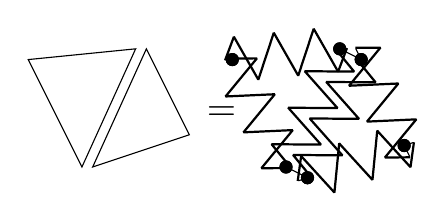
\begin{tikzpicture}[scale=0.45\columnwidth/4.0cm,every node/.style={scale=0.45\columnwidth/4.0cm}]
      \draw (0,0) -- (1,0.1) -- (0.5,-1) -- cycle;
      \draw (1.5,-0.7) -- (1.1,0.1) -- (0.6,-1) -- cycle;
      \draw (1.8,-0.5) node {=};
      \draw (1.9,0) to[R,*-*] (2.9,0.1) to[R,*-*]  (2.4,-1) to[R,*-*]  (1.9,0);
      \draw (3.5,-0.8) to[R,*-*] (3.1,0.0) to[R,*-*] (2.6,-1.1) to[R,*-*] (3.5,-0.8);
      \draw (2.9,0.1) -- (3.1,0.0);
      \draw (2.4,-1) -- (2.6,-1.1);
   \end{tikzpicture}
   }\\
\caption{%
Illustration of a 2D FEM discretization of the forward model (left, black).
Meshing is refined near electrodes to better model large gradients.
The reconstruction model mesh (left, blue) is related to the FEM by 
$\MB$. 
   First order triangular elements are equivalent to a resistor mesh (right)
with conductance $Y_{i,j} = \sigma_i \mathop{\rm cot} \alpha_{i,j}$.
}
\label{fig:FEM_mapping}
\end{figure}

The Jacobian, $\JB$, or sensitivity matrix, represents
the sensitivity of each measurement to a conductivity 
change in each image region,
\begin{equation}
\JB_{i,j} = \left. 
 \frac{\partial}
           {\partial \sG_j} F( \xB )_i 
\right|_{\sG = \sG_r}.
\end{equation}
Two approaches to calculation of $\JB$ have been used:
direct differentiation of the FEM system matrix
formulation \cite{Yorkey1987Comparing}, and
adjoint field methods \cite{Polydorides2002EIDORS},
 in which the dot (inner) product of
fields produced by stimulation and measurement patterns
are integrated over each image element.
The first requires a custom FEM solver, while the
later technique can accept the output of standard FEM algorithms.
An efficient implementation of both methods results
in the same underlying algorithm\cite{Adler2017Jacobian}.
It is also possible to approximate $\JB$ 
by making small changes in each image region, and calculate a ``perturbation
Jacobian''\TODO{REF}.  Efficient calculation of both the forward solution and
Jacobian are important to the performance of EIT solvers \cite{Boyle2012Compute}.
The perturbation approach is generally slower to execute but easiest to
implement making it suitable for validating alternate implementations.

The matrix $\JB$ may be used to investigate
aspects of an EIT system configuration. Each column
represents the change in measurements, $\partial \vB$, due to
a conductivity contrast in the corresponding FEM element, while
each row represents the relative contribution to each FEM element
from the corresponding measurement. To visualize sensitivity patterns,
the contribution from each FEM element, $i$, should be normalized by the
element size (volume, $V_i$); thus, the sensitivity, $S_i$, of EIT data to 
conductivity changes in each element $i$ is
$ S_i = (V_i)^{-1} (\sum_j J_{i,j}^2 )^{\frac{1}{2}}$.

\begin{figure} \centering
   \subcaptionbox{\centering Single measurement}[0.30\columnwidth]{\includegraphics[width=0.30\columnwidth]{../figs/sens1.png}}\hfil%
   \subcaptionbox{\centering Adjacent}[0.30\columnwidth]{\includegraphics[width=0.30\columnwidth]{../figs/sens2.png}}\hfil%
   \subcaptionbox{\centering Skip-4}[0.30\columnwidth]{\includegraphics[width=0.30\columnwidth]{../figs/sens3.png}}\\
   \centering \includegraphics[width=0.75\columnwidth]{../figs/sens-cb.png}\\
\caption{%
Spatial distributions of EIT sensitivity for various
stimulation and measurement patterns:
(a)~sensitivity to pair-drive measurement between electrodes [2,6],[3,5],
(b)~sensitivity to adjacent pattern
(c)~sensitivity to a ``skip 4'' pattern
}
\label{fig:sensitivity_patterns}
\end{figure}

While the sensitivity patterns of EIT are well understood for 
single-plane electrode placements, EIT is inherently sensitive
to off-plane conductivity contrasts (\fref{fig:off_plane_sensitivity}),
showing a ``lens-shaped'' sensitivity region.
By using a vertical placement of electrodes, it is possible to
constrain the region of sensitivity \cite{Grychtol20163DEIT}.
EIT may also be used to create 3D images \cite{Metherall1996Three},
although the reconstructions are unreliable in regions far from electrodes
as the sensitivity is very small.

\begin{figure} \centering
   \includegraphics[width=0.47\columnwidth]{../figs/fig07-offplane-sens-1plane_F.pdf}
   \includegraphics[width=0.47\columnwidth]{../figs/fig07-offplane-sens-2pl_sqF.pdf}
\caption{%
Off-plane sensititivity for a cross section through an elliptical
model of a uniform thorax, for 
(lefe)  single 32-electrode plane (skip 5), and
(right) two 16-electrodes planes  (skip 5 square pattern).
The relative sensitivity of each vertical
pixel is calculated with respect to the on-plane value, and shown by
the contours (indicating 95\%, 90\%, 75\%, 50\% and 25\% of the maximum).
}
\label{fig:off_plane_sensitivity}
\end{figure}


While sensitivity for conductivity changes is equal
for small conductive and non-conductive contrasts, the
sensitivity saturates as the magnitude of the
conductivity contrast increases.
\Fref{fig:perturbation_sensitivity} shows the 
normalized sensitivity for a cylindrical ROI in a
phantom with single electrode plane, as a function of
shape and conductivity.
 EIT is generally more sensitive
to conductive than non-conductive contrasts, and this
increased sensitivity
depends on the shape; a conductive ROI lying in the path
of current flow shows increased sensitivity.
For spherical regions, conductive contrasts have approximately
three times the sensitivity of non-conductive
ones \cite{Adler2015Perturbations}.

\begin{figure} \centering
   \includegraphics[width=0.95\columnwidth]{../figs/fig08_conductivity_contrast.pdf}
\caption{%
The relative EIT sensitivity as a function of the shape and
conductivity of an ROI. The stimulation configuration (subfigure at right)
has 16 electrodes in a central plane (dotted), and a 
has a contrasting cylindrical ROI with a height/diameter, $H$, and conductivity 
$\sigma_c$, while elsewhere $\sigma=1$.
The graph shows the
normalized EIT signal, $S(\sigma_c)$, as a function of
$\sigma_c$ for four values of $H$.
}
\label{fig:perturbation_sensitivity}
\end{figure}

\subsection{Image Reconstruction (Inverse Problem)}

Image reconstruction is an inverse problem which calculates
an estimate, $\xH$, of 
the distribution of internal properties, $\xB$, which is most consistent
with the measurements, $\yB$, and is ``reasonable'' in some sense (e.g. smoothness). 
Image reconstruction can be understood as an ``inverse sensitivity''
process, and is very poorly conditioned, since EIT is much more
sensitive to contrasts near the electrodes than in the body center.
In most cases, reconstruction is also ill-posed, because the
parameter space of $\xB$ is larger than the acquired measurements, $\yB$.


\subsubsection{Regularized Image Reconstruction}
The most common approach is based
on minimization of a norm
\begin{equation}
\| \yB - F(\xH) \|^2_\WB + \lambda^2\| \xH - \xB_0 \|^2_\QB,
\label{eqn:minimize_norm}
\end{equation}
where the first term $\yB - F(\xH)$ is the ``data mismatch''
between the measured data and their estimate via the forward model.
$\WB$ is a data weighting matrix, and represents the inverse
covariance of measurements. In most cases, $\WB$ is set to be the identity matrix;
however, given a knowledge of the reliability of each measurement channel, 
$\WB$ can be used to represent this reliability during
reconstruction \cite{Mamatjan2013Quality}.
The second term is the mismatch between the reconstruction
estimate, $\xH$, and an {\em a priori} estimate of its value, $\xB_0$.
For aEIT, $\xB_0$ is typically a uniform, homogeneous value;
accurate estimation of this value is important for convergence of aEIT
algorithms.
For difference EIT, $\xB_0=0$, since increases and decreases are
equally likely.
$\QB$ is the ``regularization matrix'' discussed later.
The relative weighting between the data and prior mismatch terms 
is controlled by a ``hyperparameter'', $\lambda$. When $\lambda$ is
large, solutions tend to be smooth and more similar to the prior;
while, for small $\lambda$, solutions have higher spatial resolution,
but are noisier and less well conditioned.

A reconstructed solution, $\xH$, minimizes (\ref{eqn:minimize_norm})
and is most commonly calculated via
an iterative update, $\xH^{(k+1)} = \xH^{(k)} + \Delta\xH^{k}$ 
starting at $\xH = \xB_0$, using
\begin{equation}
\Delta\xH^{(k)}= 
 \left( \JB_k^t \WB \JB_k + \lambda^2 \QB \right)^{-1}
       \left( \JB_k^t \WB \Delta \yB - 
      \lambda^2 \QB     \Delta \xB \right),
\label{eqn:iterative_update}
\end{equation}
where $\JB_k$ is the Jacobian, updated at each iteration based on 
$\xB^{(k)}$,
and $\Delta\yB = \yB - F(\xB^{(k)})$ 
and $\Delta\xB = \xH^{(k)} - \xH^{(0)}$.
Often, especially for tdEIT, only one iteration is required,
and a precalculated reconstruction matrix, $\RB$, can be
calculated
\begin{equation}
\xH= \left( \JB^t \WB \JB + \lambda^2 \QB \right)^{-1}
      \JB^t \WB \yB = \RB \yB
\label{eqn:linear_reconstruction}
\end{equation}
which allows for fast (real-time) reconstructions via a matrix multiplication.

Alternatively, $\RB$ may be calculated using the ``Wiener filter'' form,
which has been used by the GREIT \cite{Adler2009GREIT} algorithm. Here the
reconstruction matrix minimizes 
$\Ew[\|\yT - \RB \xT\|^2]$, where 
$\yT$ and $\xT$ correspond to the ``training'' measurements and targets
(i.e.\ representing the prior distribution of contrasts and noise), and
$\Ew[\cdot]$ is the weighted expectation operator. The reconstruction
matrix which minimizes this norm is
$\RB = \Ew[ \xT \yT^t] (\Ew[ \yT \yT^t ])^{-1}$,
which yields \cite{Grychtol20163DEIT}
\begin{equation}
\RB= \DB \SG_t \JB^t \left( \JB \SG_t \JB^t + \lambda^2 \SG_n \right)^{-1},
\label{eqn:GREIT_reconstruction}
\end{equation}
where $\DB$ maps each training location onto
a larger ``desired'' image region.
Eqn (\ref{eqn:GREIT_reconstruction}) is equivalent to 
    (\ref{eqn:linear_reconstruction}) when parameters are
selected to be the inverse covariances
$\WB = \SG_n^{-1}$ and 
$\QB = \SG_t^{-1}$, and $\DB= \IB$.

Most regularization-based algorithms use the $\ell_2$ norm in
(\ref{eqn:minimize_norm}); however, other norms
provide useful possibilities \cite{Borsic2012PDIPM}.
An $\ell_1$ norm on the 
data mismatch term provides ``robust error norms'' which
are less sensitive to outliers, while 
an $\ell_1$ norm on the image prior term (using an appropriate $\QB$)
enforces ``total variation'' regularization which has
less tendency to blur image regions.

\subsubsection{Regularization parameter selection}

The choice of regularization matrix, $\QB$, and its weighting, $\lambda$,
control the trade off in (\ref{eqn:minimize_norm}) between the
data and model mismatch, and thus the amount and type of noise
in reconstructed images. $\QB$ represents the inverse of the
covariance of the expected image (or training targets). The use
of Tikhonov regularization implies $\QB=\IB$ and assumes that
targets are independent; this choice does not work well and
results in overemphasis of boundary contrasts and a ``speckle''-type
patterns. To address the boundary overemphasis,
 regularization weighting based on the sensitivity of each element has often
been used, setting $\QB$ to the diagonal elements of $\JB^t \JB$, and has come
to be called ``NOSER regularization'' \cite{Cheney1990NOSER}.
Reduction of image speckle requires imposing a spatial filter
into $\QB$. In GREIT, this is done via a larger ``desired'' image
region and spatial correlations in the covariance, $\SG_t$. 
$\QB$ has also been designed to impose a 
high-pass spatial filter
to penalize non-smooth image content \cite{Adler1996Constrast},
\TODO{CITE Borsic}
most commonly using a Laplace filter \cite{Polydorides2002EIDORS}.

As the ``hyperparameter'', $\lambda$,
increases, the reconstructed image is constrained to be closer to
the (smooth, low-amplitude) prior model, but loses high-frequency
details. $\lambda$ is often chosen heuristically, but this means
that comparisons between algorithms are not fair, and can be
chosen in a way to hide image artefacts. Many approaches to automatically
select $\lambda$ are used \cite{Braun2017Hyperparameter}, with
criteria such as image noise or the balance of norms.
\Fref{fig:regularization_comparison} shows sample reconstructed
EIT images illustrating the effect of $\QB$ and $\lambda$ and
the reconstruction norm.

\begin{figure} \centering
% Images from
%http://eidors3d.sourceforge.net/tutorial/EIDORS_basics/tutorial120.shtml
% 
% Maybe chose an image that makes Tikhonov look worse
   \subcaptionbox{\centering Model}[0.50\columnwidth]{\includegraphics[width=0.50\columnwidth]{../figs/hp1.png}}\\
   \subcaptionbox{\centering   Tikhonov}[0.90\columnwidth]{%
      \includegraphics[width=0.30\columnwidth]{../figs/hp41.png}~~%
      \includegraphics[width=0.30\columnwidth]{../figs/hp31.png}~~%
      \includegraphics[width=0.30\columnwidth]{../figs/hp21.png}}\hfil%
   \subcaptionbox{\centering   Laplace}[0.90\columnwidth]{%
      \includegraphics[width=0.30\columnwidth]{../figs/hp42.png}~~%
      \includegraphics[width=0.30\columnwidth]{../figs/hp32.png}~~%
      \includegraphics[width=0.30\columnwidth]{../figs/hp22.png}}\hfil%
   \subcaptionbox{\centering   Noser}[0.90\columnwidth]{%
      \includegraphics[width=0.30\columnwidth]{../figs/hp43.png}~~%
      \includegraphics[width=0.30\columnwidth]{../figs/hp33.png}~~%
      \includegraphics[width=0.30\columnwidth]{../figs/hp23.png}}\hfil%
   \subcaptionbox{\centering   Total Variation}[0.90\columnwidth]{%
      \includegraphics[width=0.30\columnwidth]{../figs/hp45.png}~~%
      \includegraphics[width=0.30\columnwidth]{../figs/hp35.png}~~%
      \includegraphics[width=0.30\columnwidth]{../figs/hp25.png}}\hfil%
   \centering \includegraphics[width=0.70\columnwidth]{../figs/hp-cb.png}\\
\caption{%
EIT reconstructions as a function of hyperparameter
and regularization matrix. The top row shows the simulation model
from which tdEIT data are calculated, and Gaussian random noise
of $-12$\,dB SNR (reference the difference signal) added.
Each row shows a different choice of prior, $\QB$, while the
last row (Total Variation) also uses a $\ell_1$ norm on the model mismatch term.
Values of $\lambda$ are calculated for each $\QB$ so that noise performance
in each column is equal; noise figure values are (left column) 0.5,
(center) 1.0, 
(right) 3.0.
}
\label{fig:regularization_comparison}
\end{figure}

\subsubsection{Alternative reconstruction approaches}
The regularized reconstruction approach described in the
previous section is the most common technique; however, several
other approaches have been used. The earliest systems used
``Sheffield backprojection'' \cite{Brown1987Sheffield},
which is based on the concepts from CT filtered backprojection.
Most experimental work prior to this decade was based on this algorithm.
Another early approach used ``layer stripping'' \cite{Somersalo1991Layer}
in which ``layers'' are reconstructed moving inward from the boundary.
Backprojection and layer stripping are generally considered inappropriate for most biomedical applications.

One exciting mathematical development is the ``d-bar'' algorithm
which allows single-step nonlinear reconstruction; promising
results have been shown for simulation and (tdEIT) experimental
data  \cite{Herrera2015Direct}.
In cases where the conductivity distribution has ``jump'' changes,
a number of powerful techniques are available, such as the
monotonicity method \cite{Tamburrino2002Monotonicity} which
investigates properties of the transfer impedance map.


\subsubsection{Image validation}

Many parameters have been proposed to measure and compare
image reconstruction performance. The most basic measure
is ``distinguishability'', which is related to the signal to
noise ratio due to a contrast, and the probability with
which such contrasts can be detected given measurement
noise \cite{Isaacson1986Distinguishability, Lionheart2001Optimal}.
 Using simulation or phantom
measurements, one can calculate the
image signal to noise ratio,
amplitude response,
position error,
resolution, ringing, and shape deformation \cite{Adler2009GREIT}.
For experimental data, images can be compared to 
physiological ``knowns'' \cite{Grychtol2014Validation}.
Additionally, EIT images commonly show artefacts due
to changes at the electrodes (movement or changing contact
quality) or mismatches between instrumentation and models.
In many cases, low-quality data can be detected
and corrected \cite{Mamatjan2013Quality}
 via modifications to matrix $\WB$.
Electrode movement can be addressed to a large extent by introducing
a conductivity change Jacobian \cite{Soleimani2006Movement} in
the reconstruction formulation.


\subsection{Image Processing and EIT Measures}

Raw EIT images do not directly give relevant clinical information.
Instead images must be analysed to calculate application-relevant images
and measures. 
EIT image analysis is most developed for thoracic EIT, in which a
large number of functional EIT (fEIT) algorithms are available.
Examples are given here, and an extensive overview of fEIT techniques
is given in  \cite{Frerichs2017Chest}.

An fEIT image is calculated from  analysis of each raw image voxel
over a time-sequence
of EIT images to calculate a specific parameter. Examples are
the
``Tidal Variation'' fEIT image,
the difference between the end-inspiratory and
end-expiratory voxel values, and
the
``Expiration time'' fEIT image, representing the delay
in inspiration (or expiration) between an individual
voxel and the global waveform.




  From the processed image, specific
EIT measures may be calculated, to determine the state of the subject
and assess trends.
As an example,
\fref{fig:fEIT_eg_silent_spaces} shows the
calculation of the hypoventilated lung fEIT measure 
(introduced as ``silent spaces'' by \cite{Waldmann2015Silent}),
which represents the fraction of lung regions which receive
low or no ventilation. This EIT measure is recorded as a function of time, and
serves to assess the subject's state of ventilation.

\begin{figure} \centering
   \includegraphics[width=0.95\columnwidth]{../figs/fig10-hypoventilation-fraction.pdf}
\caption{%
Block diagram of the calculation of the
fraction of hypoventilated lung \cite{Waldmann2015Silent}.
From raw EIT images (top row), pixel waveforms are analyzed
to calculate the tidal variation (TV) fEIT image (middle row).
Within the lung ROI (identified from an anatomical atlas),
regions with less than a threshold $T=10\%$ of the maximum ventilation
are identified (bottom row) and the fraction of such pixels calculated.
}
\label{fig:fEIT_eg_silent_spaces}
\end{figure}

\TODO{
Other stuff
 - Identification of ROIs
 - Separation of cardiac and ventilation
 - estimation of timing
 - Protocol-based vs. protocol-free
}

Many other functional EIT analysis approaches have also been proposed,
and we highlight two examples.
Dynamic analysis was used by
\cite{Aristovich2014Neural}
to study
the propagaion of evoked neural activity in the cortex following
sensory stimulation.  Functional images of the activation delay
of brain regions were calculated to measure connection pathways.
The pulse propagation time between the heart and lung regions
of interest was measured by \cite{Proenca2016Noninvasive} and
shown to correlate with pulmonary arterial pressure.

For absolute imaging, EIT image processing and measures are less
well developed than for tdEIT applications. Typically, the
average reconstructed impedance in a region of interest
is compared to a threshold. For example, cancerous prostate
tissue had significantly greater conductivity than benign
regions \cite{Wan2013Transrectal}.


\section{Discussion and Perspectives}

In this review, we aim to focus
on the steps involved in interpretation
of EIT images, from the electrical properties of the
tissue (which by themselves are rarely of direct
clinical relevance) to diagnostically-useful,
EIT-based measures. With a systems-level perspective,
we hope to help clarify the relevance of components,
such as a new contact gel, electrode cofiguration on 
the body, a functional imaging protocol.
\TODO{rewrite}

In the opinion of the authors, EIT is at a time of transition.
For many of its applications, EIT is reliable
and reproducible \cite{Adler2012Whither, Frerichs2017Chest}. The
important question is whether it is relevant, in the sense that
EIT-based measures can be useful to manage patients and improve outcomes.
To be successful, EIT must provide new clinically-relevant
information which cannot be obtained, safely or conveniently, in another way.
We feel the capabilities of EIT mean it is 
best seen as {\em monitoring$++$}
 (i.e.\ an improved  monitoring technology),
rather than {\em imaging$--$}
 (i.e.\ a low-resolution imaging technology).
Using its high temporal resolution, there are rich possibilities
to explore novel fEIT modalities to extract specific physiological
information.

To achieve this, we recommend a focus on:
1) {\em availability} of EIT software (for modeling, algorithm comparison,
   and reuse) as well as reference data, possibly building on the
   EIDORS framework \cite{Adler2006EIDORS};  
2) {\em availability} of EIT devices (for phantom, animal and clinical
   use) as well as reference data;
3) {\em standards} for access to EIT data and images (such as a DICOM class)
   \TODO{ADD Ref};
4) {\rm robustness} against electrode contact errors and interference
   (automatic compensation being the most important technical 
   requirement);
5) {\em useful software} with an intuitive interface for the clinical
   and experimental user, which provides relevant parameters
   and calibrated units;
6) {\em standardized procedures} for EIT measurements indicating
   the required protocols for EIT and additional measures (e.g.\ 
   ECG, pressure) and analysis approaches;
7) {\em clinically-motivated EIT research} based on collaborations
   focused on answering specific questions.
To help further these goals, all software to create the
figures in this paper is available at {\em eidors.org/eit-review2017}.


\section{Conclusion}

EIT images internal electrical properties using
body-surface measurements; it has high temporal but low
spatial resolution, and has the advantage of being non-invasive
and potentially low cost.
It offers exciting possibilities for imaging and fuctional 
monitoring in several applications, and is currently
seeing clinical use for ventilation monitoring.
In this paper, we have reviewed the applications of
EIT with the goal to elucidate an image interpretation ``pathway''
of the process of image interpretation,
by elaborating each of the processes though which 
potentially diagnostically-relevant measures are determined
from the underlying tissue properties.
Each step from the tissue, hardware, forward \& inverse problem,
image processing and measures are described, in order
to clarify the advantages and disadvantages of various approaches.



\begin{thebibliography}{00}
      \setlength{\parskip}{0ex}% 
      \setlength{\itemsep}{0ex}% 
\bibitem{Abboud1995Peripheral}
\ifmaxthree{
M Abboud, R Guardo, R Martineau, J Taillefer, C  Pelletier, 
}{
M Abboud
}
``Monitoring of peripheral edema using electrical bioimpedance measurements''
{\em Conf IEEE EMBS} pp 641--642, 1995.

\bibitem{Adler1996Expansion}
A Adler, R Guardo, Y Berthiaume. 
``Impedance imaging of lung ventilation: do we need to account for chest expansion?''
{\em  IEEE T Biomed Eng}, 43:414--420, 1996.

\bibitem{Adler1996Constrast}
A Adler, R Guardo.
``Electrical impedance tomography: regularized imaging and contrast detection.''
{\em IEEE T Medical Imag} 15:170--179, 1996.

\bibitem{Adler2006EIDORS}
A Adler, WRB Lionheart
``Uses and abuses of EIDORS: An extensible software base for EIT''
{\em Physiol Meas} 27:S25--S42, 2006.

\bibitem{Adler2009GREIT}
\ifmaxthree{
A Adler, JH Arnold, R Bayford, A Borsic, B Brown, P Dixon, TJC Faes, I Frerichs, H Gagnon, Y Gärber, B Grychtol, G Hahn, WRB Lionheart, A Malik, RP Patterson, J Stocks, A Tizzard, N Weiler, GK Wolf
}{
A Adler
}
``GREIT: a unified approach to 2D linear EIT reconstruction of lung images''
{\em Physiol Meas}, 30:S35--S55, 2009


\bibitem{Adler2017Cerebral}
\ifmaxthree{
A Adler, M Faulkner, K Aristovich, S Hannan, J Avery, DS Holder
}{
A Adler
}
``Cerebral perfusion imaging using EIT'',
Accepted: {\em EIT 2017}, Dartmouth, NH, USA, June 21--24, 2017

\bibitem{Adler2017Sensitibity}
A Adler, A Boyle, WRB Lionheart
``Efficient computations of the Jacobian matrix using different
approaches are equivalent'',
Accepted: {\em EIT 2017}, Dartmouth, NH, USA, June 21--24, 2017


\bibitem{Adler2011Adjacent}
A Adler, PO Gaggero, Y Maimaitijiang,
``Adjacent Stimulation and Measurement Patterns Considered Harmful''
{\em Physiol Meas}, 32:731--744, 2011.


\bibitem{Adler2012Whither}
\ifmaxthree{
A Adler, MB Amato, JH Arnold, R Bayford, M Bodenstein, SH Böhm, BH Brown, I Frerichs, O Stenqvist, N Weiler, GK Wolf,
}{
A Adler
}
``Whither lung EIT: where are we, where do we want to go, and what do we need to get there?''
{\em Physiol Meas}, 33:679--694, 2012. 

\bibitem{Adler2015Hard}
A Adler, B Grychtol, R Bayford
``Why is EIT so hard, and what are we doing about it?''
{\em Physiol Meas}, 36:1067--1074. 2015.

\bibitem{Adler2015Perturbations}
A Adler, WRB Lionheart,
``Conductivity perturbations in EIT''
{\em Proc. Conf. EIT2016}, p 26, Neuchâtel, Switzerland, Jun 2--5, 2015.

\bibitem{Adler2016Handbook}
A Adler, R Gaburro, WRB Lionheart,
``Electrical Impedance Tomography'',
 in {\em Handbook of Mathematical Methods in Imaging}, 2nd ed 
O Scherzer (Ed), Springer, 2016.

\bibitem{Adler2017Jacobian}
A Adler, A Boyle, WRB Lionheart
``Efficient computations of the Jacobian matrix using different approaches are equivalent''
{\em Proc. Conf. EIT2017}, p ??, Dartmouth, USA, Jun 21--24, 2017.
\TODO{missing from EIT2017 proceedings}

\bibitem{Allaud1977}
LA Allaud, MH Martin; 
``Schlumberger, the history of a technique'',
John Wiley and Sons, New York. 1977.

\bibitem{Aristovich2014Neural}
\ifmaxthree{
KY Aristovich, GS dos Santos, BC Packham, DS Holder. 
}{
KY Aristovich
}
``A method for reconstructing tomographic images of evoked neural activity with electrical impedance tomography using intracranial planar arrays'',
{\em Physiol meas}. 35:1095--1110, 2014.

\bibitem{Assenheimer2001TScan}
\ifmaxthree{
M Assenheimer, O Laver-Moskovitz, D Malonek, D Manor, U Nahaliel, R Nitzan, A Saad
}{
M Assenheimer
}
``The T-SCANTM technology: electrical impedance as a diagnostic tool for breast cancer detection.''
{\em Physiol Meas} 22:1--8, 2001. % Feb;22(1):1.

\bibitem{Barber1983}
DC Barber, BH Brown, IL Freeston;
``Imaging Spatial distributions of resistivity using Applied Potential Tomography''.
{\em Electronics Letters} 19:93--95, 1983.

\bibitem{Barber1984}
DC Barber, BH Brown;
``Applied Potential Tomography''.
{\em  J Phys E:Sci Instrum} 17:723--733, 1984.

\bibitem{Bayford2006Bioimpendace}
RH Bayford; 
``Bioimpedance tomography (electrical impedance tomography)''
{\em Ann Rev Biomed Eng} 8:63--91, 2006.

\bibitem{Beck1996Process}
MS Beck, RA Williams,
``Process tomography: a European innovation and its applications''
{\em Meas Sci Technol} 7:215--224, 1996

\bibitem{Bodenstein2009EIT}
M Bodenstein, M David, K Markstaller;
``Principles of electrical impedance tomography and its clinical application.''
{\em Crit Care Med} 37:713--24, 2009.

\bibitem{Borcea2002EIT}
L Borcea;
``Electrical impedance tomography.''
{\em  Inverse Prob} 18:R99--R136, 2002.

\bibitem{Borsic2009Prostate}
\ifmaxthree{
A Borsic, R Halter R, Y Wan, A Hartov, KD Paulsen,
}{
A Borsic
}
``Sensitivity study and optimization of a 3D electric impedance tomography prostate probe``
{\em Physiol Meas} 30:S1--S19, 2009.

\bibitem{Borsic2012PDIPM}
A Borsic, A Adler,
``A primal dual-interior point framework for using the L1-norm or the L2-norm on the data and regularization terms of inverse problems''
{\em Inverse Prob}, 28:095011, 2012.

\bibitem{Boyle2012Compute}
A Boyle, A Borsic, A Adler,
``Addressing the computational cost of large EIT solutions''
{\em Physiol Meas} 33:787--800, 2012.

\bibitem{Braun2017Hyperparameter}
\ifmaxthree{
F Braun, M Proença, J Solà, J-P Thiran, A Adler
}{
F Braun
}
``A Versatile Noise Performance Metric for
Electrical Impedance Tomography Algorithms''
In press {\em IEEE T Biomed Eng} DOI:10.1109/TBME.2017.2659540

\bibitem{Brown1987Sheffield}
BH Brown, AD Seagar,
``The Sheffield data collection system'',
{\em Clin Phys Physiol Meas}, 8(Suppl A): 91--97, 1987.

\bibitem{Brown2003EIT}
BH Brown;
``Electrical impedance tomography (EIT): a review.''
{\em  J Med Eng Technol} 27:97--108, 2003.

\bibitem{Calderon1980}
AP Calderón,
``On an inverse boundary value problem'', in
{\em Seminar on Numerical Analysis and its Applications to Continuum Physics}, Rio de Janeiro, Editors W.H. Meyer and M.A. Raupp, Sociedade Brasileira de Matematica, pp 65--73, 1980.

\bibitem{Cheney1990NOSER}
\ifmaxthree{
M Cheney, D Isaacson, JC Newell, S Simske, J Goble.
}{
M Cheney
}
``NOSER: An algorithm for solving the inverse conductivity problem''
{\em Int J Imag Syst Technol} 2:66--75, 1990.

\bibitem{Cheney1999EIT} %% Sensitivity
M Cheney, D Isaacson, JC Newell;
``Electrical Impedance Tomography'',
SIAM Review, 41:85--101, 1999.

\bibitem{Cheng1989Complete}
\ifmaxthree{
KS Cheng, D Isaacson, JC Newell, DG Gisser DG,
}{
KS Cheng
}
``Electrode models for electric current computed tomography'',
{\em IEEE T Biomed Eng} 36:918-924, 1989.

\bibitem{Cherepenin2001Breast}
\ifmaxthree{
V Cherepenin, A Karpov, A Korjenevsky, V Kornienko, A Mazaletskaya, D Mazourov, D Meister
}{
V Cherepenin
}
``A 3D electrical impedance tomography (EIT) system for breast cancer detection.''
{\em Physiol Meas} 22:9--18, 2001. % Feb;22(1):9.

\bibitem{Choi2007Mammography}
\ifmaxthree{
MH Choi, TJ Kao, D Isaacson, GJ Saulnier, JC Newell
}{
MH Choi
}
``A reconstruction algorithm for breast cancer imaging with electrical impedance tomography in mammography geometry.''
{\em IEEE T Biomed Eng} 54:700-10, 2007. % Apr;54(4):700-10.

\bibitem{Costa2009EIT}
EL Costa, RG Lima, MB Amato MB;
``Electrical impedance tomography.''
{\em Curr Opin Crit Care} 15:18--24, 2009.

\bibitem{Coulombe2005Parametric}
\ifmaxthree{
N Coulombe, H Gagnon, F Marquis, Y Skrobik, R Guardo
}{
N Coulombe
}
``A parametric model of the relationship between EIT and total lung volume.''
{\em  Physiol Meas} 26:401--411, 2005.


\bibitem{Dijkstra1993EIT}
\ifmaxthree{
AM Dijkstra, BH Brown, AD Leathard, ND Harris, DC Barber, DL Edbrooke,
}{
AM Dijkstra
}
``Review clinical applications of electrical impedance tomography''
{\em J Medical Eng Technol}, 17:89--98, 1993.

\bibitem{Frerichs2000EIT}
I Frerichs;
``Electrical impedance tomography (EIT) in applications related to lung and ventilation: a review of experimental and clinical activities.''
{\em  Physiol Meas} 21:R1--R21, 2000.

\bibitem{Frerichs2002Perfusion}
\ifmaxthree{
I Frerichs, J Hinz, P Herrmann, G Weisser, G Hahn, M Quintel, G Hellige.
}{
I Frerichs
}
``Regional lung  perfusion  as  determined  by  electrical
  impedance  tomography  in  comparison  with  electron beam CT imaging''
{\em IEEE T Med Imag} 21:646--652, 2002.

\bibitem{Frerichs2014EIT}
I Frerichs, T Becher, N Weiler; 
``Electrical impedance tomography imaging of the cardiopulmonary system.''
{\em Curr Opin Crit Care} 20:323--32, 2014.

\bibitem{Frerichs2017Chest}
\ifmaxthree{
I Frerichs, M Amato, A Van Kaam, D Tingay, Z Zhao, B Grychtol, M Bodenstein,
H; Gagnon, S Böhm, E Teschner, O Stenqvist, T Mauri, V Torsani, C Luigi,
A Schibler, G Wolf, D Gommers, S Leonhardt, A Adler
}{
I Frerichs
}
``Chest electrical impedance tomography
examination, data analysis, terminology, clinical use and recommendations:
consensus statement of the TRanslational EIT developmeNt stuDy group''
{\em Thorax}, 72:83--93, 2017.


\bibitem{Gabriel1996Dielectric}
S Gabriel, RW Lau, C Gabriel,
``The dielectric properties of biological tissues: III. Parametric models for the dielectric spectrum of tissues'',
{\em  Phys Med Biol} 41:2271--2293, 1996.

\bibitem{Gabriel2009Frequencies}
C Gabriel, A Peyman, EH Grant,
{\em Electrical conductivity of tissue at frequencies below 1 MHz}
{\em Phys Med Biol} 54:4863--4878, 2009.

\bibitem{Geselowitz1971Reciprocity}
DB Geselowitz, 
``An application of electrocardiographic lead theory to impedance
plethysmography''
{\em  IEEE T Biomed Eng} 1:38--41, 1971.

\bibitem{Gomez2012Overdistension}
C Gómez-Laberge, JH Arnold, GK Wolf
``A Unified Approach for EIT Imaging of Regional Overdistension and Atelectasis
in Acute Lung Injury'',
{\em IEEE T Medical Imag}, 31:834--842, 2012.

\bibitem{Grychtol2012Mismatch}
\ifmaxthree{
B Grychtol, WRB Lionheart, M Bodenstein, GK Wolf, A Adler
}{
B Grychtol
}
``Impact of model shape mismatch on reconstruction quality in Electrical Impedance Tomography''
{\em IEEE T Medical Imag}, 31:1754--1760, 2012.

\bibitem{Grychtol2013Refinement}
B Grychtol, A Adler,
``FEM electrode refinement for Electrical Impedance Tomography''
{\em Conf IEEE EMBS} pp 6429--6432, 2013. %Osaka, Japan, July 3--7, 2013.

\bibitem{Grychtol2014Validation}
\ifmaxthree{
B Grychtol, G Elke, P Meybohm, N Weiler, I Frerichs, A Adler,
}{
B Grychtol
}
``Functional Validation and Comparison Framework for EIT Lung Imaging''
{\em PLoS ONE} 9:e103045, 2014.

\bibitem{Grychtol20163DEIT}
B Grychtol, B Müller, A Adler,
``3D EIT image reconstruction with GREIT'',
{\em Physiol Meas} 37:785--800, 2016.

\bibitem{Halter2007Postate}
\ifmaxthree{
RJ Halter, A Hartov, JA Heaney, KD Paulsen, AR Schned
}{
RJ Halter
}
``Electrical impedance spectroscopy of the human prostate.''
{\em IEEE T Biomed Eng} 54:1321-7, 2007. % Jul;54(7):1321-7.

\bibitem{Hartinger2007Hardware}
AE Hartinger, H Gagnon, R Guardo,
``Accounting for hardware imperfections in EIT image reconstruction algorithms''
{\em  Physiol Meas} 28:S13--S27,2007

\bibitem{Henderson1978}
RP Henderson, JG Webster;
``An Impedance Camera for Spatially Specific Measurements of the Thorax''
{\em IEEE T Biomed Eng} 25:250--254, 1978.

\bibitem{Herrera2015Direct}
\ifmaxthree{
CN Herrera, MF Vallejo, JL Mueller, RG Lima;
}{
CN Herrera
}
``Direct 2-D reconstructions of conductivity and permittivity from EIT data on a human chest.''
{\em IEEE T Med Imag}, 34:267--74, 2015.

\bibitem{Hoetink2004Flow}
\ifmaxthree{
AE Hoetink, TJ Faes, KR Visser, RM Heethaar,
}{
AE Hoetink
}
``On the flow dependency of the electrical conductivity of blood''
{\em  IEEE T Biomed Eng} 51:1251--1261, 2004.

\bibitem{Holder1992Ischaemia}
DS Holder,
``Electrical impedance tomography with cortical or scalp electrodes during global cerebral ischaemia in the anaesthetised rat.''
{\em Clin Phys Physiol Meas} 13:87--98, 1992. % Feb;13(1):87.

\bibitem{Holder2004Book}
DS Holder, ed;
``Electrical impedance tomography: methods, history and applications.''
CRC Press, 2004.


\bibitem{Hua1991Optimal}
\ifmaxthree{
P Hua, EJ Woo, JG Webster,  WJ Tompkins,
}{
P Hua
}
``Iterative reconstruction methods using regularization and optimal current patterns in electrical impedance tomography''
{\em  IEEE T Med Imag} 10:621--628, 1991.

\bibitem{IEC60601}
IEC 60601-1:2015,
 ``Medical Electrical Equipment Part 1:  General Requirements for
Basic Safety and Essential Performance'',
Brussels: International Electrotechnical Commission, 2015

\bibitem{Isaacson1989Optimal}
D Goble, D Isaacson.
``Optimal current patterns for three-dimensional electric current computed tomography''
{\em Conf. IEEE EMBS} pp 463--464, 1989.

\bibitem{Isaacson1986Distinguishability}
D Isaacson;
``Distinguishability of conductivities by electric current computed tomography.''
{\em IEEE T Med Imag} 5: 91--95, 1986.

\bibitem{Jossinet1998Breast}
J Jossinet,
``The impedivity of freshly excised human breast tissue''
{\em Physiol Meas} 19:61--75, 1998.

\bibitem{Kerner2002Spectroscopy}
\ifmaxthree{
TE Kerner, KD Paulsen, A Hartov, SK Soho, SP Poplack,
}{
TE Kerner
}
``Electrical impedance spectroscopy of the breast: clinical imaging results in 26 subjects.''
{\em  IEEE T Med Imag} 21:638--645, 2002.

\bibitem{Khan2015FPGA}
\ifmaxthree{
S Khan, P Manwaring, A Borsic, R Halter, 
}{
S Khan
}
``FPGA-based voltage and current dual drive system for high frame rate electrical impedance tomography''
{\em IEEE T Medical Imag}, 34:888--901, 2015.

\bibitem{Larsson2007Quasistatic}
J Larsson,
``Electromagnetics from a quasistatic perspective'',
{\em Am J Physics} 75:230-239, 2007.

\bibitem{Leonhardt2011Bladder}
\ifmaxthree{
S Leonhardt, A Cordes, H Plewa, R Pikkemaat, I Soljanik, K Moehring, HJ Gerner, R Rupp,
}{
S Leonhardt
}
``Electric impedance tomography for monitoring volume and size of the urinary bladder.''
{\em Biomedizinische Technik} 56:301--307, 2011

\bibitem{Leonhardt2012EIT}
S Leonhardt, B Lachmann;
``Electrical impedance tomography: the holy grail of
ventilation and perfusion monitoring?''
{\em Int Care Med} 38:1917-1929, 2012.

\bibitem{Li1996Active}
JH Li, C Joppek, U Faust,
``Fast EIT data acquisition system with active electrodes and its application to cardiac imaging''
{\em  Physiol Meas}. 17:A25--A32, 1996.

\bibitem{Lee1989Anisotopic}
JM Lee, G Uhlmann, ``Determining anisotropic real-analytic
 conductivities by boundary measurements,''
{\em Comm. Pure Appl. Math.} 42:1097--1112, 1989.

\bibitem{Lionheart2001Optimal}
WRB Lionheart, J Kaipio, CN McLeod;
``Generalized optimal current patterns and electrical safety in EIT.'' 
{\em Physiol Meas} 22: 85--90, 2001.

\bibitem{Lionheart2010Finite}
WRB Lionheart, K Paridis,
``Finite elements and anisotropic EIT reconstruction''
{\em  J Phys: Conf Ser} 224:012022, 2010.

\bibitem{Lorentz1896Reciprocity}
HA Lorentz,
``The theorem of Poynting concerning the energy in the electromagnetic
field and two general propositions concerning the propagation of light''
{\em  Amsterdammer Akademie der Wetenschappen} 4:176--??, 1896.
\TODO{end page number missing}


\bibitem{Lozano1995Prolonged}
Lozano A, Rosell J, Pallas-Areny R. 
``Errors in prolonged electrical impedance measurements due to electrode repositioning and postural changes.''
{\em  Physiol Meas} 16:121--130, 1995.

\bibitem{Lundin2012EIT}
S Lundin, O Stenqvist;
``Electrical impedance tomography: potentials and pitfalls.''
{\em Curr Opin Crit Care} 18:35--41, 2012.


\bibitem{Mamatjan2013Quality}
\ifmaxthree{
Y Mamatjan, B Grychtol, P Gaggero, J Justiz, V Koch, A Adler. 
}{
Y Mamatjan
}
``Evaluation and Real-Time Monitoring of Data Quality in Electrical Impedance Tomography''.
{\em IEEE T Med Imaging} 32:1997--2005, 2013.

\bibitem{Mangnall1987}
\ifmaxthree{
YF Mangnall, AJ Baxter, R Avill, NC Bird, BH Brown, DC Barber, AD Seagar, AG Johnson, NW Read
}{
YF Mangnall
}
``Applied potential tomography: a new noninvasive technique for assessing gastric function'',
{\em Clin Phys Physiol Meas}, 8:119-129 1987.

\bibitem{Metherall1996Three}
\ifmaxthree{
P Metherall, DC Barber, RH Smallwood, BH Brown.
}{
P Metherall
}
``Three dimensional electrical impedance tomography''
{\em Nature} 380:509-512, 1996.

\bibitem{Newell1996}
\ifmaxthree{
JC Newell, PM Edic, X Ren, JL Larson-Wiseman, MD Danyleiko,
}{
JC Newell
}
``Assessment of acute pulmonary edema in dogs by electrical impedance imaging.''
{\em  IEEE T Biomed Eng} 43:133--138, 1996.

\bibitem{Nguyen2012Perfusion}
\ifmaxthree{
DT Nguyen, C Jin, A Thiagalingam, AL McEwan
}{
DT Nguyen
}
``A review on electrical impedance tomography for pulmonary perfusion imaging.''
{\em Physiol Meas} 33:695--706, 2012.

\bibitem{Nissinen2009Errors}
\ifmaxthree{
A Nissinen, LM Heikkinen, V Kolehmainen, JP Kaipio
}{
A Nissinen
}
``Compensation of errors due to discretization, domain truncation and unknown contact impedances in electrical impedance tomography''
{\em  Meas Sci Technol}. 20:105504, 2009.

\bibitem{Packham2012Frequency}
\ifmaxthree{
B Packham, H Koo, A Romsauerova, S Ahn, A McEwan, SC Jun, DS Holder,
}{
B Packham
}
``Comparison of frequency difference reconstruction algorithms for the detection of acute stroke using EIT in a realistic head-shaped tank''
{\em Physiol Meas} 33:767--786, 2012.



\bibitem{Polydorides2002EIDORS}
N Polydorides, WRB Lionheart. 
``A Matlab toolkit for three-dimensional electrical impedance tomography: a contribution to the Electrical Impedance and Diffuse Optical Reconstruction Software project.''
{\em Meas Sci Technol} 13:1871--1883, 2002.

\bibitem{Proenca2015Motion}
\ifmaxthree{
M Proença, F Braun, M Rapin, J Solà, A Adler, B Grychtol, S Böhm, M Lemay, J-P Thiran,
}{
M Proença
}
``Influence of heart motion on cardiac output estimation by means of electrical impedance tomography: a case study''
{\em Physio. Meas}, 36:1175--1192, 2015.

\bibitem{Proenca2016Noninvasive}
\ifmaxthree{
M Proença, F Braun, J Solà, A Adler,
M Lemay, J-P Thiran, SF Rimoldi
}{
M Proença
}
``Non-invasive monitoring of pulmonary artery pressure from timing information by EIT: experimental evaluation during induced hypoxia''
{\em Physiol Meas} 37:713--726, 2016.

\bibitem{Rapin2015Cooperative}
\ifmaxthree{
M Rapin, M Proença, F Braun, J Solà, O Chételat,
}{
M Rapin
}
``Cooperative sensors: a new approach towards wearable EIT systems'',
{\em Proc. Conf. EIT2016}, p 44, Neuchâtel, Switzerland, Jun 2--5, 2015.

\bibitem{Riedel2010EIT}
T Riedel, I Frerichs;
``Electrical impedance tomography.''
{\em Eur  Respir  Mon} 47:195--205, 2010.

\bibitem{Romsauerova2006mfEIT}
\ifmaxthree{
A Romsauerova, A McEwan, L Horesh, R Yerworth, RH Bayford, DS Holder
}{
A Romsauerova
}
``Multi-frequency electrical impedance tomography (EIT) of the adult human head: initial findings in brain tumours, arteriovenous malformations and chronic stroke, development of an analysis method and calibration.''
{\em Physiol Meas} 27:S146--S161, 2006. % Apr 20;27(5):S147.

\bibitem{Roth2015Correlation}
\ifmaxthree{
CJ Roth, A Ehrl, T Becher, I Frerichs, JC Schittny, N Weiler, WA Wall, 
}{
CJ Roth
}
``Physiological Measurement
Correlation between alveolar ventilation and 
electrical properties of lung parenchyma''
{\em Physiol Meas} 36: 1211--1226, 2015

\bibitem{Sadleir2009blood}
\ifmaxthree{
RJ Sadleir, T Tang, AS Tucker, P Borum, M Weiss
}{
RJ Sadleir
}
``Detection of intraventricular blood using EIT in a neonatal piglet model.''
{\em Conf IEEE EMBS} pp 3169-3172, 2009.

\bibitem{Schuessler1995Esophageal}
TF Schuessler, JHT Bates, 
``Utility of an esophageal reference electrode for thoracic electrical impedance tomography''
{\em Conf. IEEE EMBS} pp 559--560, 1995

\bibitem{Seo2008fdEIT}
\ifmaxthree{
JK Seo, J Lee, SW Kim, H Zribi, EJe Woo;
}{
KJ Seo
}
``Frequency-difference electrical impedance tomography (fdEIT): algorithm development and feasibility study'',
{\em  Physiol Meas} 29:929--944, 2008.


\bibitem{Silvera2015Skin}
\ifmaxthree{
David Silvera-Tawil ; David Rye ; Manuchehr Soleimani ; Mari Velonaki
}{
D Silvera-Tawil
}
Electrical Impedance Tomography for Artificial Sensitive Robotic Skin: A Review
{\em IEEE Sensors J}, 15:2001--2016, 2015.

\bibitem{Sola2011Central}
\ifmaxthree{
J Solà, A Adler, A Santos, G Tusman, FS Sipmann, SH Böhm,
}{
J Solà
}
``Non-invasive monitoring of central blood pressure by Electrical Impedance
Tomography (EIT): first experimental evidence''
{\em Med Biol Eng Comput}, 49:409--415, 2011.

\bibitem{Soleimani2006Ultrasound}
Soleimani M, ``Electrical impedance tomography imaging using a priori ultrasound data.''
{\em Biomedical engineering online} 5, 2006. % Feb 6;5(1):8.
DOI:10.1186/1475-925X-5-8

\bibitem{Soleimani2006Movement}
M Soleimani, C Gómez-Laberge, A Adler.
``Imaging of conductivity changes and electrode movement in EIT'',
{\em Physiol Meas} 27:S103--S113, 2006.

\bibitem{Somersalo1991Layer}
\ifmaxthree{
E Somersalo, M Cheney, D Isaacson, E Isaacson. 
}{
E Somersalo
}
``Layer stripping: a direct numerical method for impedance imaging.''
{\em Inverse Prob} 7:899--926, 1991.

\bibitem{Sylvester1986Uniqueness}
J Sylvester, G Uhlmann,
``A uniqueness theorem for an inverse
boundary value problem n electrical prospection''
{\em Comm Pure Appl Math} 3991-3112, 1986.

\bibitem{Tamburrino2002Monotonicity}
A Tamburrino, G Rubinacci,
``A new non-iterative in version method in electrical resistance tomography'',
{\em Inverse Prob}, 18:1809-1829, 2002.

\bibitem{Trepte2016Edema}
\ifmaxthree{
CJC Trepte, CR Phillips, J Solà, A Adler, SA Haas, M Rapin; SH Böhm, DA Reuter
}{
CJC Trepte
}
``Electrical impedance tomography (EIT) for quantification of pulmonary edema in acute lung injury'',
{\em Crit Care},  20:18, 2016.

\bibitem{Trepte2017StrokeVolume}
\ifmaxthree{
CJC Trepte, C Phillips, J Solà, A Adler, B Saugel, S Haas, SH Böhm, DA Reuter
}{
CJC Trepte}
``Electrical impedance tomography (EIT) for non-invasive assessment of stroke volume variation in health and experimental lung injury''
{\em Br J Anaesthesia}, 118:68--76, 2017.

\bibitem{Uhlmann2009EIT}
G Uhlmann;
``Electrical impedance tomography and Calderón's problem.''
{\em  Inverse Prob}.25:123011, 2009.

\bibitem{Vogt2016Heterogeneity}
\ifmaxthree{
B Vogt, K Ehlers, V Hennig, Z Zhao, N Weiler, I Frerichs;
}{
B Vogt
}
``Heterogeneity of regional ventilation in lung-healthy adults'',
{\em Proc.~Conf.~EIT2016}, p.106, 
Stockholm, Sweden, Jun 19--23, 2016.

\bibitem{vonkNoordegraaf2000}
\ifmaxthree{
A Vonk-Noordegraaf, A Janse, JT Marcus, JGF Bronzwaer, PE Postmus, TJC Faes, PMJM de Vries,
}{
A Vonk-Noordegraaf
}
``Determination of stroke volume by means of electrical impedance tomography''
{\em Physiol Meas} 21:285--293, 2000 

\bibitem{Waldmann2015Silent}
\ifmaxthree{
AD Waldmann, PL Róka, SH Böhm, W Windisch, S Strassmann, C Karagiannidis.
}{
AD Waldmann
}
``Assessment of silent spaces at different PEEP levels by electrical impedance tomography in severe COPD''.
{\em Int Care Med Experimental} 3:A456, 2015.

\bibitem{Waldmann2017Interface}
\ifmaxthree{
AD Waldmann, KH Wodack, A März, A Ukere,
CJ Trepte, SH Böhm, DA Reuter
}{
AD Waldmann
}
``Performance of novel patient interface for electrical impedance
tomography applications''
In press: {\em J Medical Biol Eng}, 2017.

\bibitem{Wan2013Transrectal}
\ifmaxthree{
Y Wan, A Borsic, J Heaney, J Seigne, A Schned, M Baker, S Wason, A Hartov, R Halter
}{
Y Wan
}
``Transrectal electrical impedance tomography of the prostate: Spatially coregistered pathological findings for prostate cancer detection''
{\em Medical physics} 40:063102, 2013.

\bibitem{Wolf2013Mechanical}
\ifmaxthree{
GK Wolf, C Gómez-Laberge, JS Rettig, SO Vargas, CD Smallwood, SP Prabhu, SH Vitali, D Zurakowski, JH Arnold
}{
GK Wolf
}
``Mechanical ventilation guided by electrical impedance tomography in experimental acute lung injury.''
{\em Crit Care Med} 41:1296-304, 2013. % May 1;41(5):1296-304.

\bibitem{Yorkey1987Comparing}
TJ Yorkey, JG Webster, WJ Tompkins,
``Comparing reconstruction algorithms for electrical impedance tomography''
{\em  IEEE T Biomed Eng} 11:843--852, 1987.

\end{thebibliography}
\end{document}

\section{Extra stuff}

\subsection{Validity of Electrostatic approximation}

The current density, $\JV$, and electric field, $\EV$,
in the body are related by Ohm's law, $\JV = \sigma \EV$,
where $\sigma(\xV, t)$ is the isotropic tissue conductivity
and varies as a function of space and time. For anisotropic
tissue, a $\sigma$ becomes a tensor. Since $\EV$ varies
sinusoidally with the drive current, it can be represented
as a phasor and a complex $\sigma$ at the drive frequency is
used. Continuity requires
$\nabla \cdot \JV = \frac{\partial}{\partial t}\rho$,
but in a conductor charge does not accumulate, so $\rho=0$.
The quasi-static approximation requires that 
$\nabla \times \EV = -\frac{\partial}{\partial t}\BV ~\approx 0$,
in which case the electric field
 can be described by a voltage, $V$, 
$\EV = - \nabla  V$, so the voltage
within a body is determined by the 
Laplace (or Poisson's) equation $\nabla \cdot \sigma V = 0$.

Validity:
https://ocw.mit.edu/courses/electrical-engineering-and-computer-science/6-007-electromagnetic-energy-from-motors-to-lasers-spring-2011/lecture-notes/MIT6_007S11_lec17.pdf

\subsection{References}

